
In this section, the obtained results from a Gaussian mixture training are reviewed. Two out of three frameworks are succesfully tested in this model.

In both frameworks \texttt{Breast Cancer} database is used with the main goal of learning a Gaussian mixture model, the original database and the one obtained via a dimensionality reduction. The latter is done using a variational auto-encoder with \texttt{InferPy}, showing that frameworks can be used together.

\section{InferPy}

Firstly, the Gaussian mixture cannot be directly modeled using \texttt{InferPy} due to the fact that \texttt{TensorFlow} \texttt{-Probability} name categorical variables as \texttt{NOT\_REPARAMETERIZED}, which, citing its documentation means that ``samples from the distribution are not fully reparameterized, and straight-through gradients are either partially unsupported or are not supported at all''. Unsuccessful attempts have being made using \texttt{MixtureGaussian} distribution available in \texttt{InferPy}, which encapsulates the mixture without needed explicit categorical variables. In this attempts, parameters that must remain positive reach negatives values even using a \texttt{softplus} filter, which makes inference not possible.

Adding a constant term to those parameters, such as, \(0.1\) in an attempt to keep them positive resulted in no learning errors but also no real results, where even the component weight parameter remained nearby its prior value on Breast Cancer database (where it should tend to \([0.63,\ 0.37]\)).


\section{Scikit-Learn}

Because of the high number of parameters, models are defined with \texttt{covariance\_type = ``diag''}, which means that all covariance matrix are diagonal. Using \texttt{``full''} covariance matrix would mean that two \(30 \times 30\) matrices might be learned from only \(569\) datapoints. Doing this reduction, the amount of covariance parameters is reduced to \(2\times 30 = 60\).

One of the parameters that can be easily studied when dealing with \(30\) parameters is the weight of each component:

\begin{minted}{python}
  print(gm.weights_)
\end{minted}

Which resulted in \([0.31003524\ 0.68996476]\) after the training and is more accurate than the prior value (\(0.5\) each).

\texttt{Scikit-Learn} allows to compute the posterior probability of belonging to each component by the usage of \texttt{gm.predict\_proba(points)}. This might be applied to each class, showing how it is distributed over the components, an ideal result would be that each of the classes is totally governed by each component. Function \texttt{plot\_mixture\_distplot} computes the posterior probabilities for each class, showing a density function fitting this results. Figure~\ref{fig:proba_ob} shows this density functions over the original dataset.

\begin{figure}[h!]
  \centering
  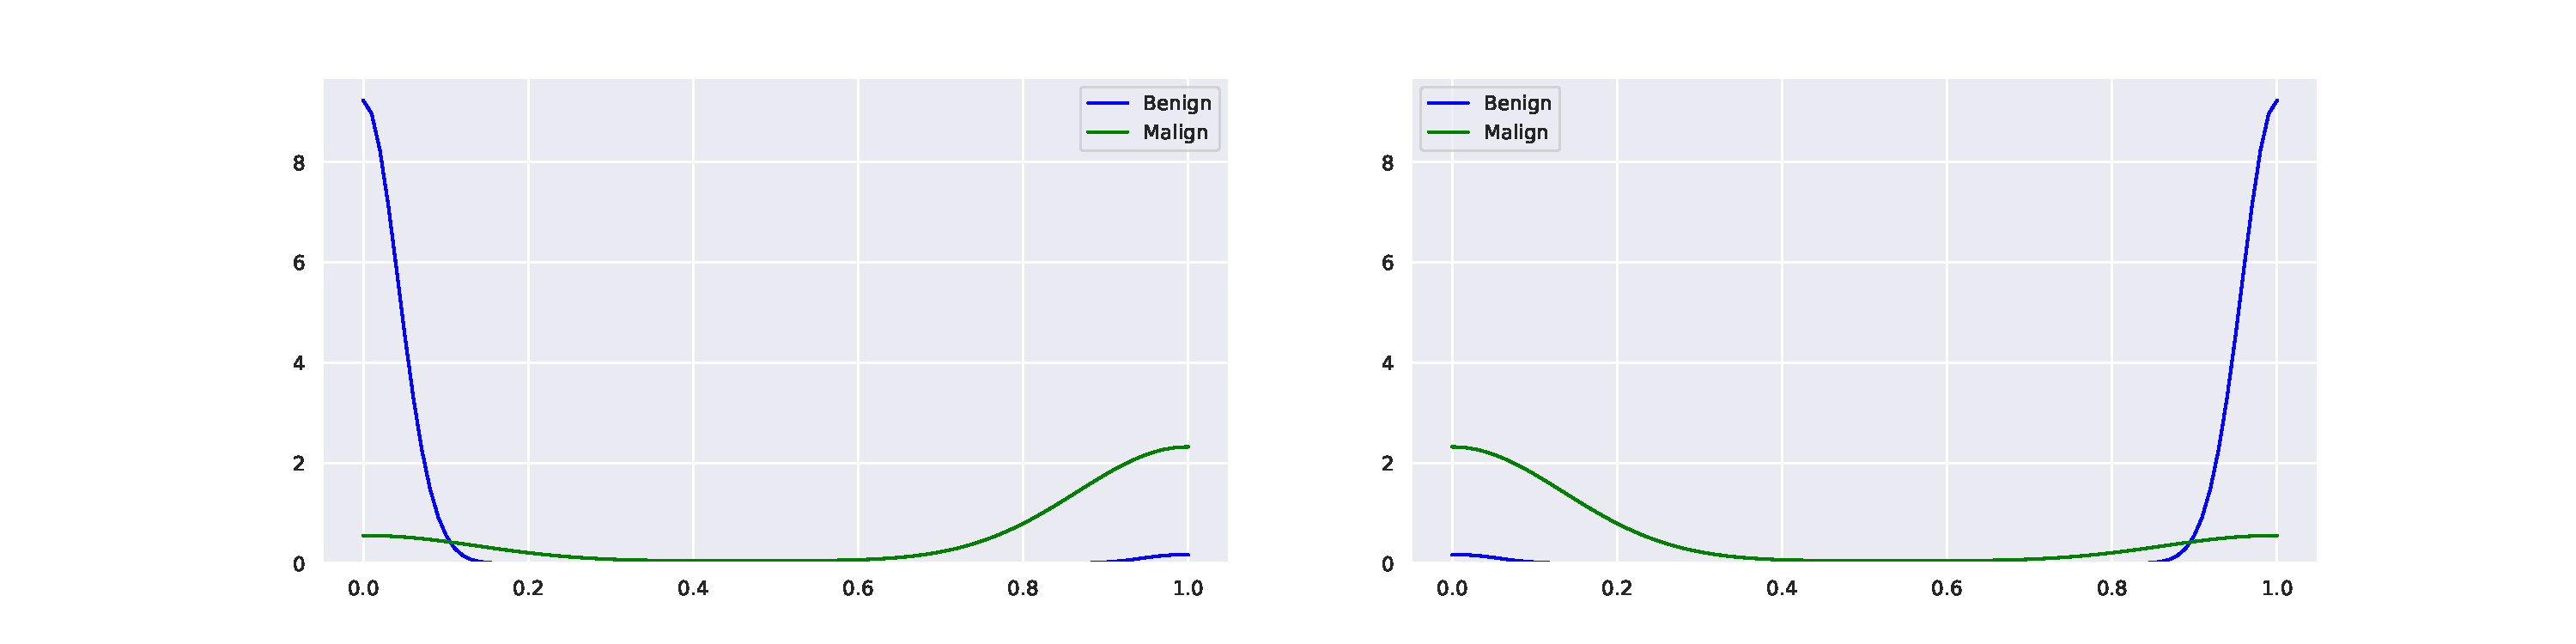
\includegraphics[width=0.9\textwidth]{tex/images/proba_observed.pdf}
  \caption{Component belonging density.}\label{fig:proba_ob}
\end{figure}

One may see that benign cases are almost completely modeled by the second component whereas the malign ones are more distributed but still modeled by the first component.

The dataset is now reduced to a three-dimensional representation using a variational auto-encoder, the dimensionality of the middle layer is \(100\) and \(4000\) epochs are used. The obtained reduction is shown in Figure~\ref{fig:vae_mix_breast}. The obtained component belonging densities are shown in
Figure~\ref{fig:proba_red} on the reduced space, showing a sharper density on the benign class compared to the original data, meaning that this class is better represented by the component in the reduced space.

\begin{figure}[h!]
    \centering
    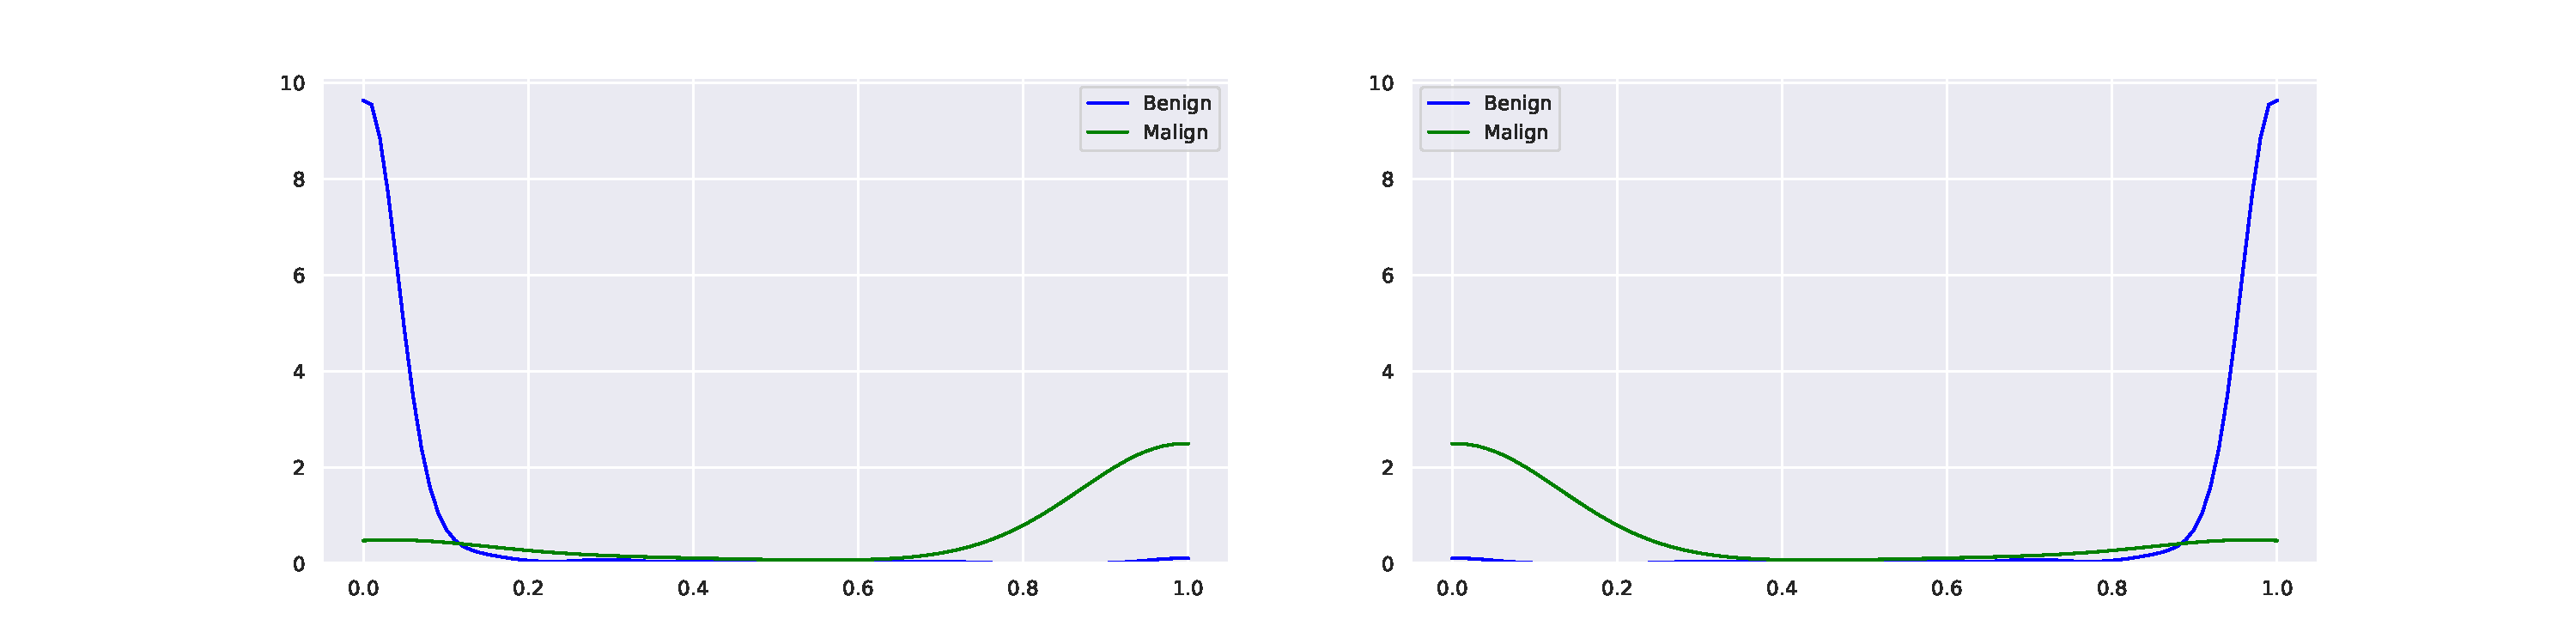
\includegraphics[width=0.9\textwidth]{tex/images/proba_reduced.pdf}
    \caption{Component belonging density in reduced data.}\label{fig:proba_red}
\end{figure}


\begin{figure}[h!]
  \centering
  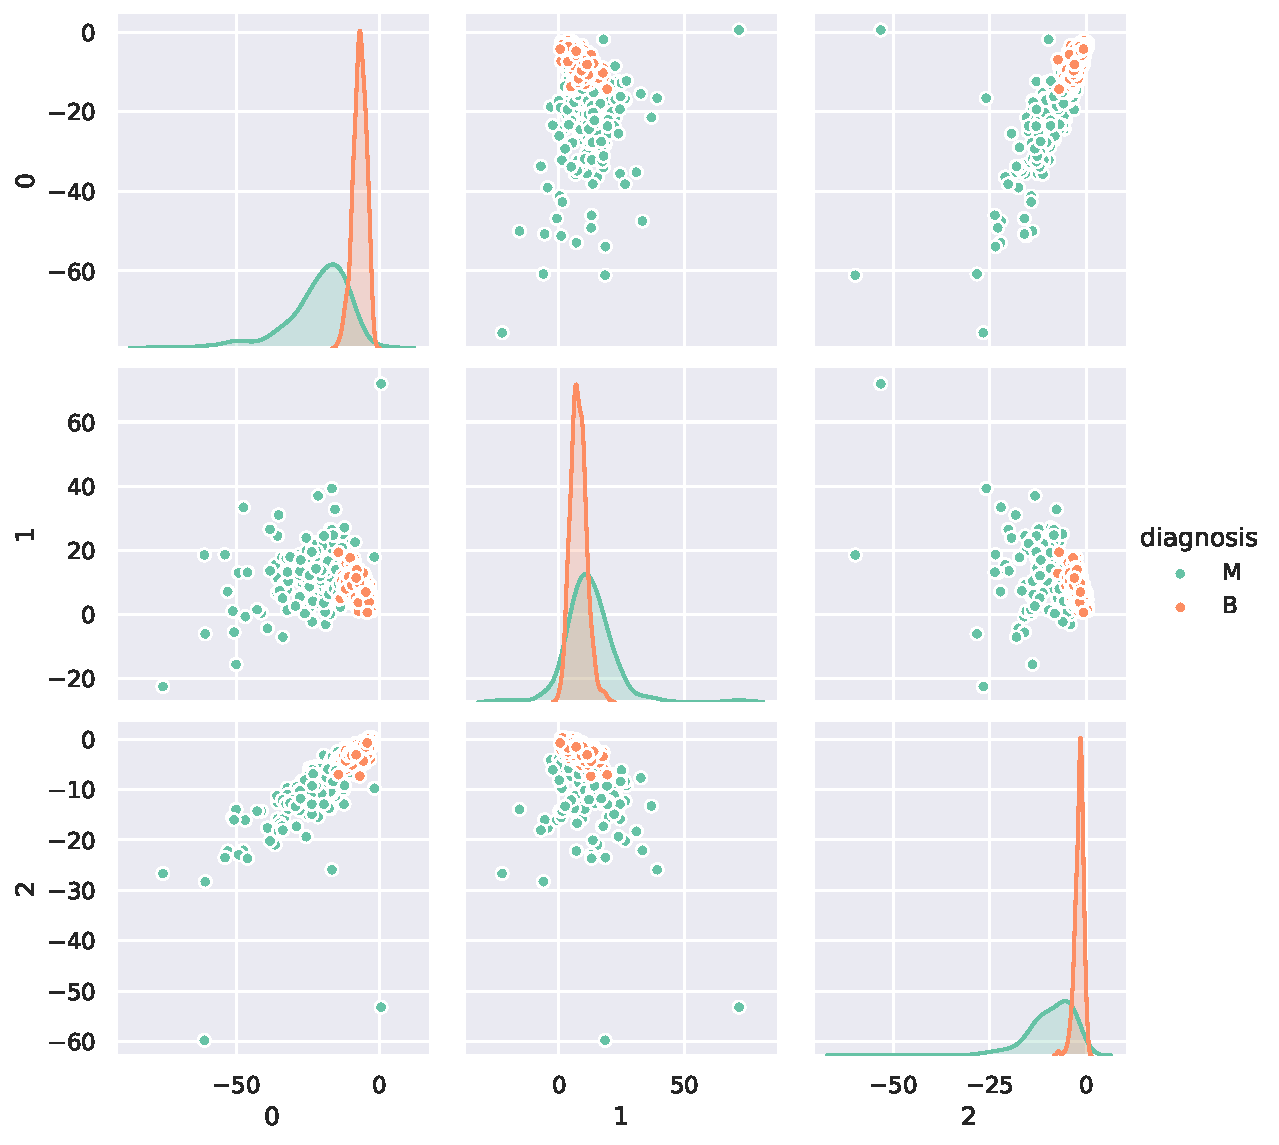
\includegraphics[width=0.9\textwidth]{tex/images/breast_vae_3D_mixture.pdf}
  \caption{Breast Cancer two-dimensional reduction representation. Reduction made trough a variational auto-encoder.}\label{fig:vae_mix_breast}
\end{figure}

As the representation is three-dimensional it is easy to compare other parameters as the mean value of each component, these are \([ 16.15134999,\  -3.88342216,\ -18.26021824]\) and \([7.25244497,\   1.90782194,\  -5.72329033]\). Using this values and Figure~\ref{fig:vae_mix_breast}, one may notice that the first component seeks to model the malign points and the second the benign ones.

\newpage
\section{BayesPy}

The \texttt{BayesPy} model can be easily created using the syntax explained before, the model parameters are initialized as
\begin{itemize}
  \item The means variable $\mu$ follows a centered normal distribution:
  $$\mu_k \sim \mathcal{N}_{data\_dim}(0,I).$$
  \item The precision variables $\Lambda$ follow a Wishart distribution with parameters:
  $$\Lambda_k \sim \mathcal{W}_{data\_dim}(data\_dim, I).$$
  \item The weights concentration variable follows a Dirichlet with parameter:
  $$ \pi \sim \text{Symmetric-Dirichlet}\Big(\frac{1}{n\_classes}\Big).$$
\end{itemize}

Which is coded as the following.
\begin{minted}{python}
    Lambda = nodes.Wishart(dim, np.identity(dim), plates=(n_components,))
    mu = nodes.Gaussian(np.zeros(dim), np.identity(dim), plates=(n_components,))
    pi = nodes.Dirichlet(np.ones(n_components)/n_components)
    z = nodes.Categorical(pi, plates=(n_samples,))
    x = nodes.Mixture(z, nodes.Gaussian, mu, Lambda)
\end{minted}

Due to the high number of attributes (784) in \texttt{Mnist} database, \texttt{BayesPy} is not able to handle the VMP algorithm with a great number of samples (it attempts to locate a matrix with shape \((n\_samples,\ n\_components,\ 784,\ 784)\)). For this reason, \texttt{Breast Cancer} is used.

The model is created with the same number of components as different classes (2) in an attempt to learn one Gaussian distribution for each class. After the inference task, \texttt{BayesPy} provides a way to inspect each variable posterior by simply printing the desired variable.

Variable moments are also accessible via each variable \texttt{u} parameter, given this, we may learn each data-point component belonging posterior, using \texttt{Z's} first moment.

The obtained results show a model that does not learn the two classes, despite that, almost all data-points belong to one of the components with high probability. The exact posterior for \(\bpi\) is \([6.5/570\  563.5/570]\).  Figure~\ref{fig:proba_original_bayes} shows each class component belonging, one may see that not proper densities are shown due to the fact that all benign points belong to the second component with probability 1.

\begin{figure}[h!]
  \centering
  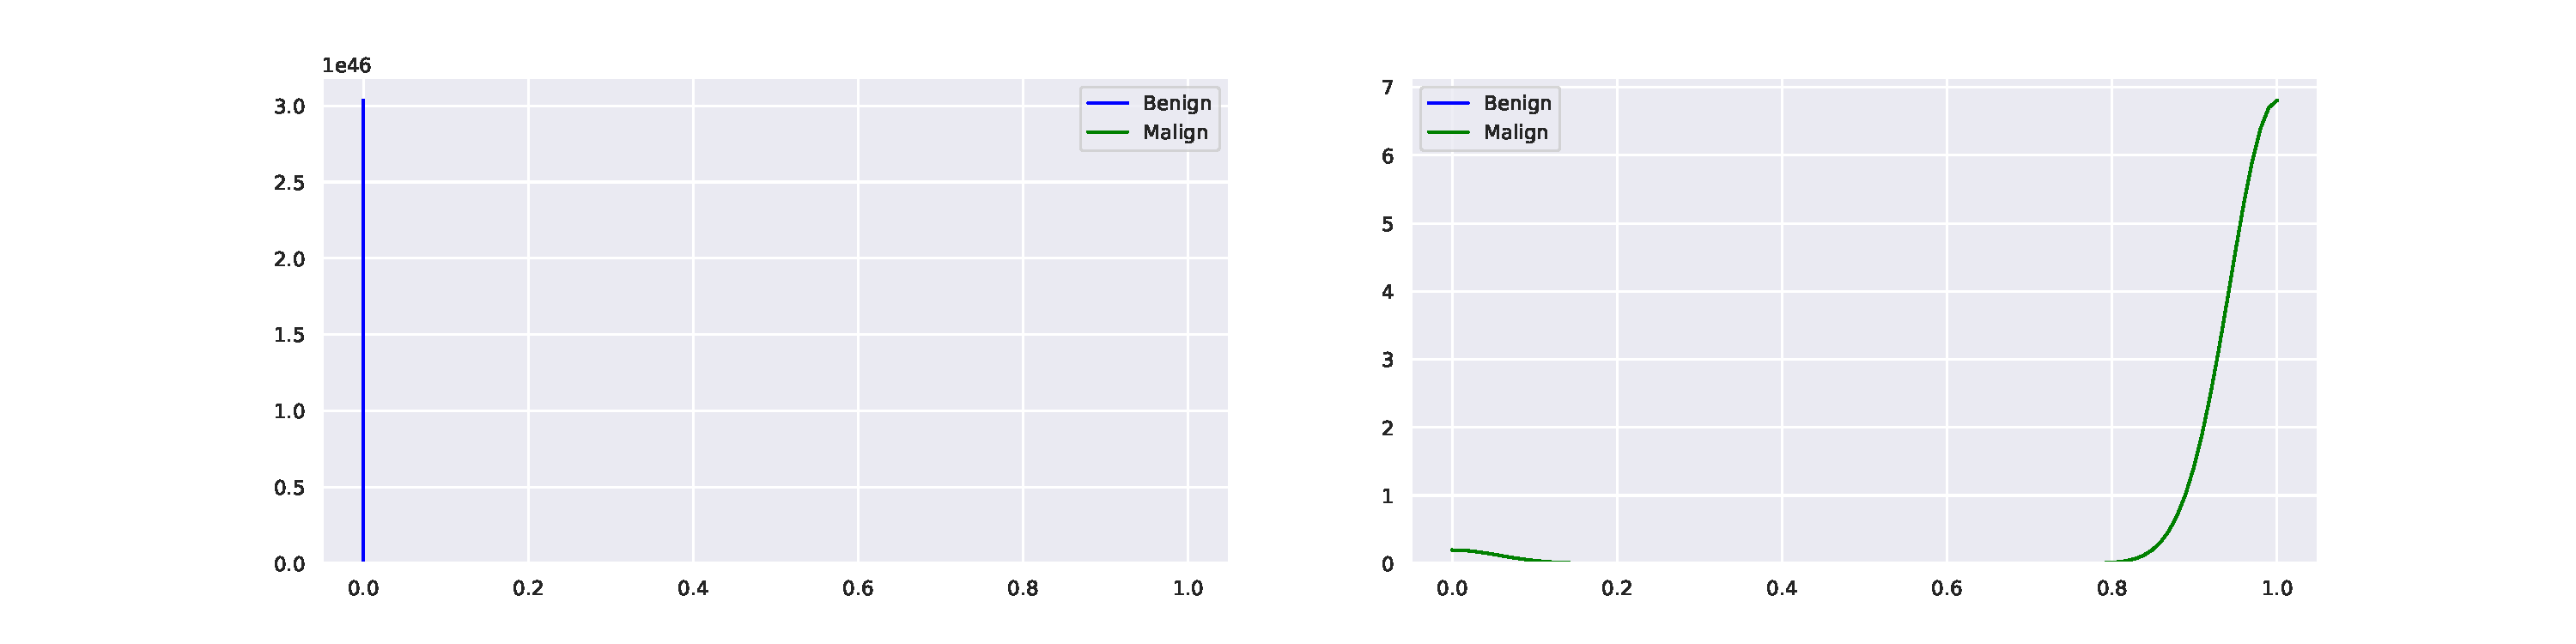
\includegraphics[width=0.9\textwidth]{tex/images/proba_original_bayes.pdf}
  \caption{Component belonging density in original data.}\label{fig:proba_original_bayes}
\end{figure}

We may reduce the space to a two-dimensional one, using a variational auto-encoder, leading to a more uniform result (Figure~\ref{fig:proba_reduced_bayes}). This is more similar to the ones obtained using \texttt{Scikit-Learn}.
 
\begin{figure}[h!]
  \centering
  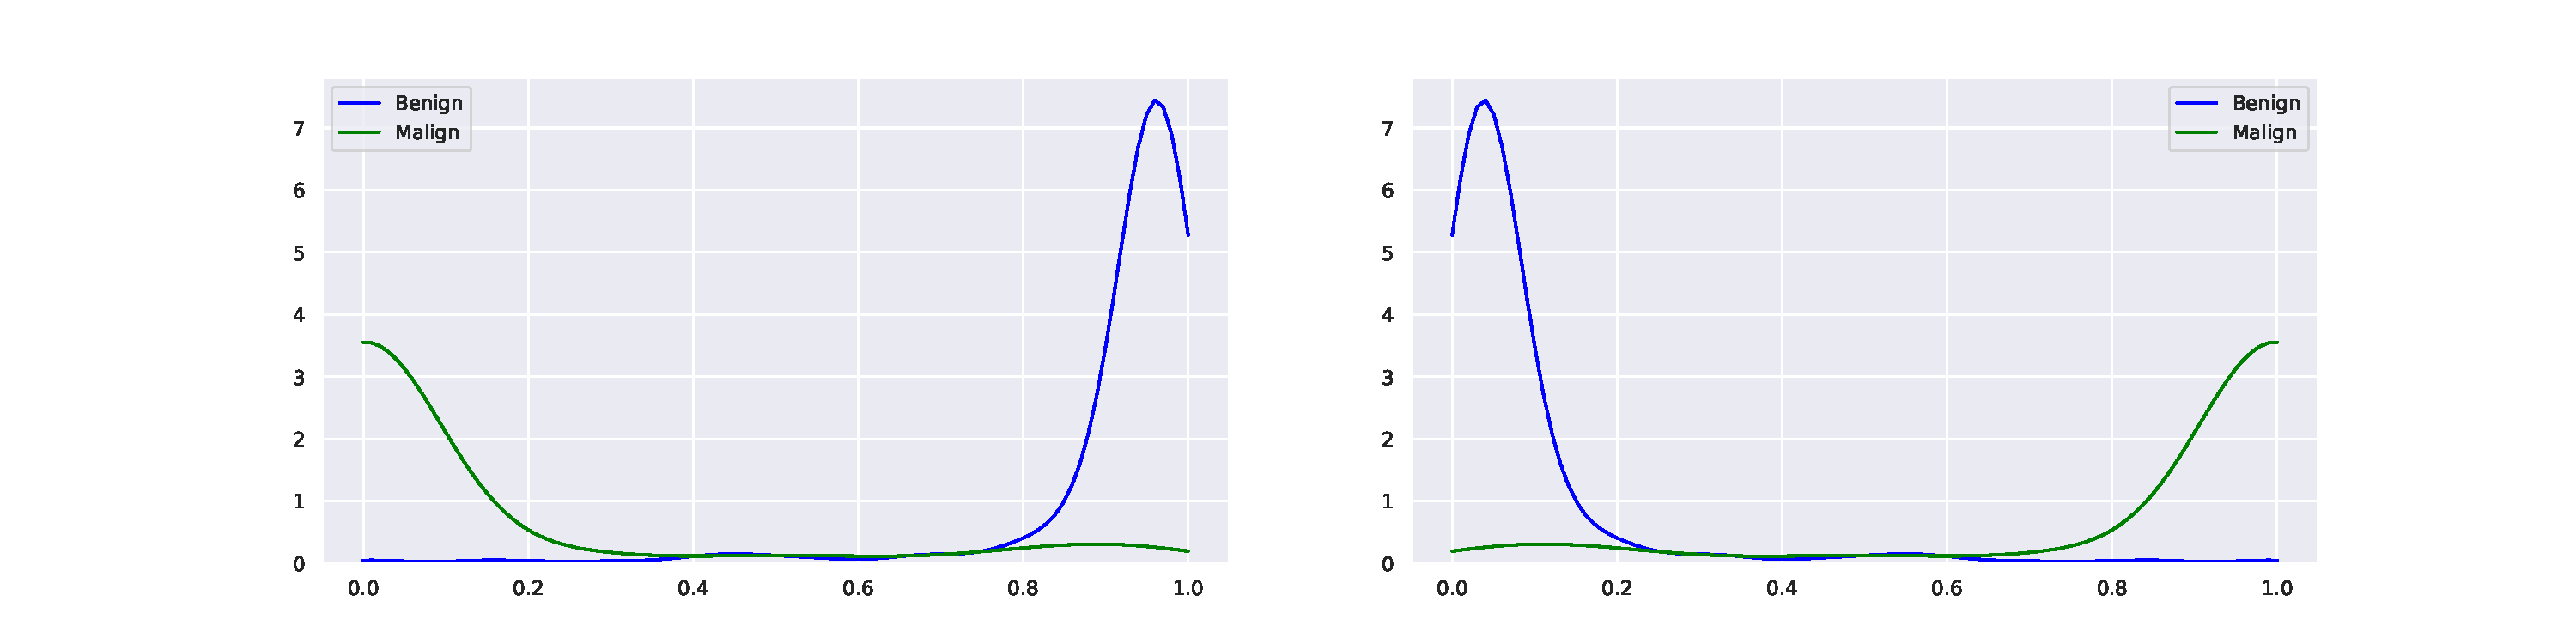
\includegraphics[width=0.9\textwidth]{tex/images/proba_reduced_bayes.pdf}
  \caption{Component belonging density in reduced data.}\label{fig:proba_reduced_bayes}
\end{figure}

\texttt{BayesPy} allows to print the learned Gaussian components using its own plotting function \texttt{gaussian\_mixture\_2d}, in Figure~\ref{fig:bayespy_red_cancer} one may see the reduced dataset along with one of the Gaussian ellipses. Unsuccessful attempts have being made to get both ellipses in the figure.

\begin{figure}[h!]
  \centering
  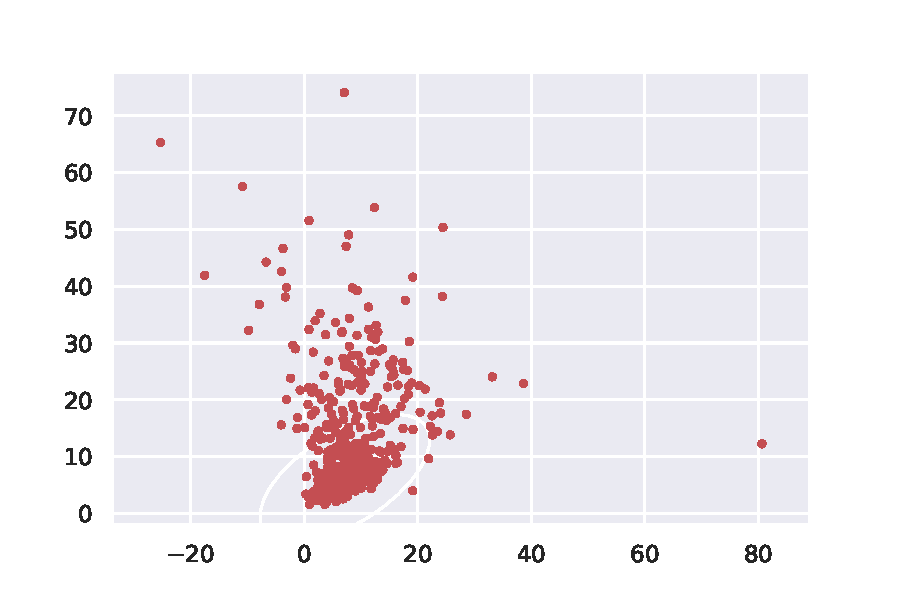
\includegraphics[width=0.9\textwidth]{tex/images/bayespy_cancer_red.pdf}
  \caption{Component belonging density in reduced data.}\label{fig:bayespy_red_cancer}
\end{figure}
